\documentclass{beamer}

% Frame Number
\setbeamertemplate{footline}[frame number]

% Input Encoding
\usepackage[utf8]{inputenc}

% PDF Bookmarks
\usepackage{url}
\usepackage{hyperref} 
\hypersetup{colorlinks}
\hypersetup{bookmarksopen}
\hypersetup{bookmarksnumbered}
\hypersetup{citecolor=blue}
\hypersetup{urlcolor=blue}
\hypersetup{linkcolor=blue}

% Spacing
\usepackage{xspace}

% Figures
\usepackage{graphicx}
\graphicspath{{../../img/}}
\usepackage{subcaption}

% Tables
\usepackage{booktabs}

% Strike Through
\usepackage{ulem}

% Code Snippet 
\usepackage{listings}
\lstset{
  belowcaptionskip=1\baselineskip,
  breaklines=true,
  frame=L,
  xleftmargin=\parindent,
  numbers=left,
  stepnumber=2,
  language=C,
  tabsize=2,
  showstringspaces=false,
  basicstyle=\footnotesize\ttfamily,
  keywordstyle=\bfseries\color{blue},
  commentstyle=\itshape\color{gray},
  identifierstyle=\bfseries\color{black},
  stringstyle=\bfseries\color{purple},
}

% Title
\title[Nanvix]{%
	\textbf{%
		The Nanvix Operating System\\
		\small{Page Replacement}
	}
}

% Authors
\author[Pedro H. Penna]{%
	Pedro H. Penna%
}

% Affiliations
\institute{
	\url{pedrohenriquepenna@gmail.com}
}

% Short-Hands
\newcommand{\ie}{\textit{ie.\xspace}}

\begin{document}

\frame{\titlepage}

\section{Background on Page Replacement}

	\begin{frame}
	\frametitle{Virtual Memory}
	\framesubtitle{Fundamentals}
		\begin{itemize}
		\setlength\itemsep{1.5em}
			\uncover<1->{
				\item Multiprogramming
				\begin{itemize}
				\setlength\itemsep{0.5em}
					\item Segmentation
					\item Paging
					\item Segmentation + Paging
				\end{itemize}
			}
			\uncover<2->{
				\item Virtual memory
				\begin{itemize}
					\item Swapping
					\item Page replacement
				\end{itemize}
			}
		\end{itemize}
	\end{frame}

	\begin{frame}
	\frametitle{Page Replacement}
	\framesubtitle{Classical Algorithms}
		\begin{itemize}
		\setlength\itemsep{1.5em}
			\uncover<1->{
				\item First in First Out (FIFO)
			}
			\uncover<2->{
				\item Second Chance (Clock)
			}
			\uncover<3->{
				\item Not Recently Used (NRU)
			}
			\uncover<4->{
				\item Least Recently Used (LRU)
				\begin{itemize}
					\item Not Frequently Used (NFU)
					\item Aging
				\end{itemize}
			}
			\uncover<5->{
				\item Working Set + Clock (WSclock)
			}
		\end{itemize}
	\end{frame}

\section{Page Replacement  in Nanvix}

	\begin{frame}
	\frametitle{Page Replacement in Nanvix}
	\framesubtitle{Paging Subsystem}
		\begin{itemize}
		\setlength\itemsep{1.5em}
			\uncover<1->{
				\item Two-level paging scheme
			}
			\uncover<2->{
				\item Global-policy frame allocation
			}
			\uncover<3->{
				\item Local page replacement
			}
			\uncover<4->{
				\item No load control
			}
			\uncover<5->{
				\item Demand paging 
			}
			\uncover<6->{
				\item Copy-on-write
			}
		\end{itemize}
	\end{frame}

	\begin{frame}
	\frametitle{Page Replacement in Nanvix}
	\framesubtitle{Virtual Address Translation}
		\begin{figure}
			\centering
			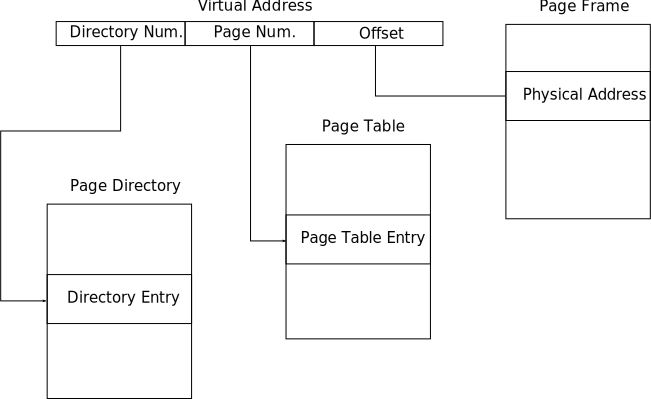
\includegraphics[width=0.9\linewidth]{paging}
			\caption{Virtual address translation in Nanvix.}
		\end{figure}
	\end{frame}

	\begin{frame}
	\frametitle{Page Replacement in Nanvix}
	\framesubtitle{Current Implementation}
		\begin{itemize}
		\setlength\itemsep{1.0em}
			\uncover<1->{
				\item Page table entry -- \texttt{struct pte}
				\begin{itemize}
				\setlength\itemsep{0.5em}
					\item \texttt{include/i386/paging.h}
				\end{itemize}
			}
			\uncover<2->{
				\item Frame allocation -- \texttt{allocf()}
				\begin{itemize}
				\setlength\itemsep{0.5em}
					\item \texttt{src/kernel/mm/paging.c}
				\end{itemize}
			}
			\uncover<3->{
				\item Validity page faults -- \texttt{vfault()}
				\begin{itemize}
				\setlength\itemsep{0.5em}
					\item \texttt{src/kernel/mm/paging.c}
				\end{itemize}
			}
			\uncover<4->{
				\item Clock interrupt handler -- \texttt{do\_clock()}
				\begin{itemize}
				\setlength\itemsep{0.5em}
					\item \texttt{src/kernel/arch/arch/x86.c}
				\end{itemize}
			}
			\uncover<5->{
				\item FIFO page replacement
				\begin{itemize}
				\setlength\itemsep{0.5em}
					\item Account when pages were brought in
					\item Evict the oldest page
				\end{itemize}
			}
		\end{itemize}
	\end{frame}

\end{document}
